\documentclass[margin=5mm]{standalone}
\usepackage[dvipsnames]{xcolor}
\usepackage{pgfplots}
\usepackage{tikz}
\usepackage[tikz]{ocgx2}

\pgfplotsset{compat=1.18}
\begin{document}

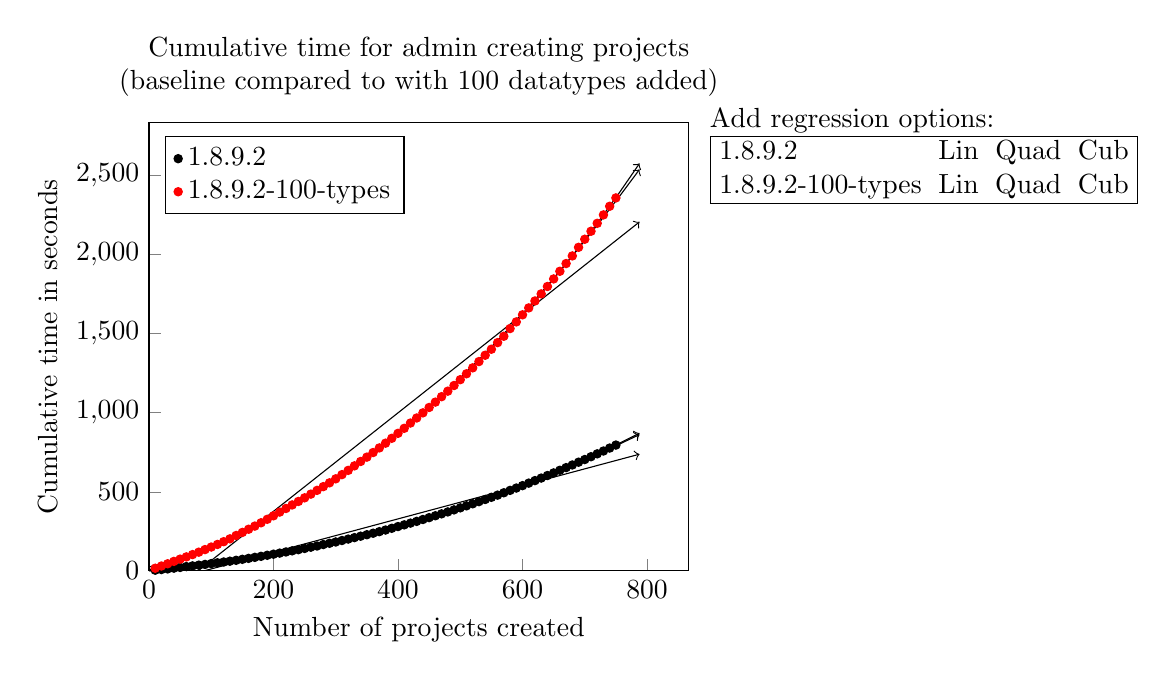
\begin{tikzpicture}
    \begin{axis}[
        align = center,
        legend pos = north west,
        legend cell align = left,
        xlabel = Number of projects created,
        ylabel = Cumulative time in seconds,
        xtick pos = left,
        ytick pos = left,
        scaled ticks = false,
        xmin = 0,
        ymin = 0,
        title = {Cumulative time for admin creating projects (baseline compared to with 100 datatypes added)},
        title style = {text width = 0.8\textwidth},
        legend entries={\switchocg{1.8.9.2}{1.8.9.2},\switchocg{1.8.9.2-100-types}{1.8.9.2-100-types}}]
        \begin{scope}[ocg = {ref = 1.8.9.2-Lin, status = invisible}]
            \plot[domain=0:788,->,forget plot] (\x,{-92.722935135135031714526121504604816436767578125 + 1.0543007766714078687897426789277233183383941650390625*(\x)^1});
        \end{scope}
        \begin{scope}[ocg = {ref = 1.8.9.2-Quad, status = invisible}]
            \plot[domain=0:788,->,forget plot] (\x,{8.2841235098111294377076774253509938716888427734375 + 0.267232787230268609146577318824711255729198455810546875*(\x)^1 + 0.0010356157755804468005578211631245721946470439434051513671875*(\x)^2});
        \end{scope}
        \begin{scope}[ocg = {ref = 1.8.9.2-Cub, status = invisible}]
            \plot[domain=0:788,->,forget plot] (\x,{2.142996908140947454057823051698505878448486328125 + 0.3611035404357758604731998275383375585079193115234375*(\x)^1 + 0.00072886619507744171940488708827388109057210385799407958984375*(\x)^2 + 0.00000026907857938860109233821719769419456014247771236114203929901123046875*(\x)^3});
        \end{scope}
        \begin{scope}[ocg = {ref = 1.8.9.2, status = visible}]
            \addplot[
                only marks,
                color = black,
                mark = *,
                mark size = 1.5 pt
            ]coordinates {(10,4.751)(20,8.862)(30,12.96)(40,17.612)(50,22.097)(60,27.513)(70,32.021)(80,36.607)(90,41.098)(100,46.356)(110,51.529)(120,56.519)(130,61.744)(140,67.213)(150,73.49)(160,79.452)(170,85.888)(180,92.402)(190,99.097)(200,105.912)(210,112.755)(220,119.873)(230,127.099)(240,134.397)(250,142.15)(260,150.194)(270,157.718)(280,166.823)(290,174.88)(300,183.078)(310,192.363)(320,201.393)(330,210.59)(340,219.767)(350,228.952)(360,238.36)(370,248.218)(380,258.558)(390,269.624)(400,280.544)(410,291.293)(420,302.319)(430,313.378)(440,325.15)(450,336.875)(460,348.858)(470,360.904)(480,373.115)(490,386.008)(500,398.791)(510,411.563)(520,424.613)(530,438.074)(540,451.632)(550,465.439)(560,479.138)(570,494.169)(580,509.199)(590,523.933)(600,539.166)(610,555.034)(620,571.039)(630,587.036)(640,603.108)(650,619.582)(660,636.422)(670,653.234)(680,669.755)(690,687.307)(700,704.251)(710,721.963)(720,740.222)(730,758.099)(740,776.644)(750,795.58)};
        \end{scope}
        \begin{scope}[ocg = {ref = 1.8.9.2-100-types-Lin, status = invisible}]
            \plot[domain=0:788,->,forget plot] (\x,{-245.475428108107990965436329133808612823486328125 + 3.11171638975817899108733399771153926849365234375*(\x)^1});
        \end{scope}
        \begin{scope}[ocg = {ref = 1.8.9.2-100-types-Quad, status = invisible}]
            \plot[domain=0:788,->,forget plot] (\x,{24.908404324323793588291664491407573223114013671875 + 1.004829383791176145024337529321201145648956298828125*(\x)^1 + 0.0027722197446934256602479873521360786980949342250823974609375*(\x)^2});
        \end{scope}
        \begin{scope}[ocg = {ref = 1.8.9.2-100-types-Cub, status = invisible}]
            \plot[domain=0:788,->,forget plot] (\x,{-0.96139487844020210527418157653301022946834564208984375 + 1.4002645692143651512395763347740285098552703857421875*(\x)^1 + 0.00148002198231758359640852784622211402165703475475311279296875*(\x)^2 + 0.00000113350680910161627493377457798207075256868847645819187164306640625*(\x)^3});
        \end{scope}
        \begin{scope}[ocg = {ref = 1.8.9.2-100-types, status = visible}]
            \addplot[
                only marks,
                color = red,
                mark = *,
                mark size = 1.5 pt
            ]coordinates {(10,17.174)(20,31.208)(30,45.38)(40,60.3)(50,74.703)(60,88.775)(70,103.473)(80,118.668)(90,135.024)(100,151.077)(110,167.564)(120,184.972)(130,202.822)(140,224.195)(150,243.47)(160,263.558)(170,283.431)(180,304.452)(190,326.426)(200,348.519)(210,372.003)(220,394.702)(230,417.266)(240,439.27)(250,462.178)(260,485.534)(270,509.344)(280,532.883)(290,557.041)(300,582.225)(310,608.93)(320,635.628)(330,664.168)(340,691.973)(350,719.344)(360,748.368)(370,777.605)(380,807.609)(390,838.433)(400,869.838)(410,901.503)(420,934.921)(430,966.728)(440,999.26)(450,1033.239)(460,1067.154)(470,1101.468)(480,1136.369)(490,1172.082)(500,1208.916)(510,1246.269)(520,1283.723)(530,1323.413)(540,1363.342)(550,1401.408)(560,1443.167)(570,1483.415)(580,1532.028)(590,1574.174)(600,1618.932)(610,1662.598)(620,1706.473)(630,1751.141)(640,1797.999)(650,1845.663)(660,1894.172)(670,1942.973)(680,1991.192)(690,2045.497)(700,2096.673)(710,2147.139)(720,2197.293)(730,2250.553)(740,2305.055)(750,2357.795)};
        \end{scope}
    \end{axis}
    \begin{scope}
        \addtolength{\tabcolsep}{-0.3em}
        \node [below right, shape=rectangle, align=left](regressiontable) at (7,6) {
            Add regression options: \\
            \begin{tabular}{|llll|}
                \hline
                1.8.9.2 & \switchocg{1.8.9.2-Lin}{Lin} & \switchocg{1.8.9.2-Quad}{Quad} & \switchocg{1.8.9.2-Cub}{Cub} \\
                1.8.9.2-100-types & \switchocg{1.8.9.2-100-types-Lin}{Lin} & \switchocg{1.8.9.2-100-types-Quad}{Quad} & \switchocg{1.8.9.2-100-types-Cub}{Cub} \\
                \hline
            \end{tabular}
        };
    \end{scope}
\end{tikzpicture}

\end{document}